\subsection{Vision Transformer}\label{s:vit}
\chapterauthor{Low Hong Sheng Jovian (2203654)}

Vision Transformers (ViT) mark a crucial adaptation of transformer architectures from textual to image analysis \cite{Khan2021Transformers}. Initially designed for natural language processing, transformers employ self-attention mechanisms which are adeptly applied to visual data in ViTs. This adaptation enables the model to dynamically prioritize different image segments according to their relevance for tasks like tumor detection in brain MRI scans.

ViTs work by breaking down an image into fixed-size patches, embedding them linearly, and treating each as a token, similar to words in text processing \cite{Wu2020Visual} (see Figure \ref{fig:vit_architecture}). Positional embeddings are added to maintain spatial relationships. These embeddings are processed through multiple transformer layers, utilizing self-attention to analyze the image holistically, enhancing the detection of complex patterns and subtle nuances indicative of tumors.

\begin{figure}[H]
  \centering
  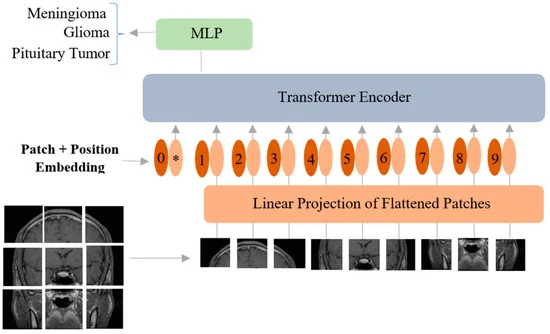
\includegraphics[width=0.45\textwidth]{vit/vit_architecture.png}
  \caption{ViT Architecture \cite{curroncol29100590}}
  \label{fig:vit_architecture}
\end{figure}

This method allows ViTs to excel in scenarios requiring deep contextual understanding and detailed image analysis. Particularly in medical imaging, ViTs are highly effective, often surpassing conventional CNNs by identifying less obvious features crucial for accurate diagnostics \cite{Matsoukas2021Is}.

Additionally, ViTs benefit from transfer learning, where models pre-trained on extensive general datasets are fine-tuned for specific medical tasks \cite{Simon2022Vision}. This not only reduces the need for large medical datasets but also speeds up the training process. Their adaptability and prowess in handling intricate image data make Vision Transformers a promising advancement in medical diagnostics, especially for improving the accuracy and reliability of brain tumor classifications.

\subsubsection{Vision Transformer Data Preprocessing}

In the initial stages of this project, several preprocessing steps were considered to optimize the performance of the ViT model for brain MRI classification. Typically, the ViT model benefits from breaking down images into smaller patches, as this allows the self-attention mechanism to effectively capture local and global features within the image. For this reason, the dataset was initially preprocessed to create patches from 224x224 pixel images. This preprocessing included resizing, cropping, normalization, and dividing the images into smaller patches.

However, during experimentation, it was observed that this approach did not yield the desired performance improvements. Specifically, the model's accuracy and ability to generalize did not improve significantly when using patched images. This was likely due to the relatively small size of the dataset, which limited the model's capacity to effectively learn from the patches. Furthermore, using the typical 16x16 patch size for ViT models resulted in a substantial increase in computational complexity \cite{Wang2021Not}. Each 224x224 pixel image was split into 196 patches, and with a total dataset size of 480 images, the resulting number of patches became unmanageable for training on available resources such as Google Colab. This immense volume of patches overwhelmed the system's memory and processing capabilities, significantly hindering the training process.

Consequently, it was decided to simplify the preprocessing approach and use the pretrained ViT model directly on the original 224x224 pixel images. This decision was made to balance computational efficiency and model performance, ensuring that the training process remained feasible given the hardware constraints and dataset size.


\subsubsection{Implementation}

The proposed brain MRI classification model employs the ViT architecture, specifically the B16 variant, pretrained on the ImageNet dataset. The Vision Transformer represents a significant departure from traditional convolutional neural network models like InceptionV3, U-Net, and ResNet-50, primarily through its utilization of self-attention mechanisms. These mechanisms enable ViT to effectively capture and interpret the global context of an image, a capability that proves particularly valuable in the domain of medical image analysis, such as MRI scans. Unlike conventional models that rely on local receptive fields, ViT assesses all parts of the image in relation to one another, enhancing the detection and classification of nuanced features within complex medical images.

To specifically tailor the ViT model for brain MRI classification, several key adjustments were made. Initially, an input size of 512x512 pixels was used; however, this did not result in good performance of the model. Consequently, the input size was adjusted to 224x224 pixels with three channels, aligning with the common dimensions of medical imaging datasets. The B16 variant of the Vision Transformer was employed without its original classification head. The transformer's outputs undergo Global Average Pooling to condense the feature maps into a singular 768-dimensional vector, effectively capturing essential features while reducing dimensionality. To mitigate overfitting, a Dropout layer with a rate of approximately 0.328 was incorporated. A dense layer containing 512 neurons, activated by ReLU, leads to a final classification layer consisting of four neurons, each corresponding to a different brain tumor class. 

The implemented architecture of the proposed model is visually represented in Figure \ref{fig:vit_implemented_architecture}. 


\begin{figure}[H]
  \centering
  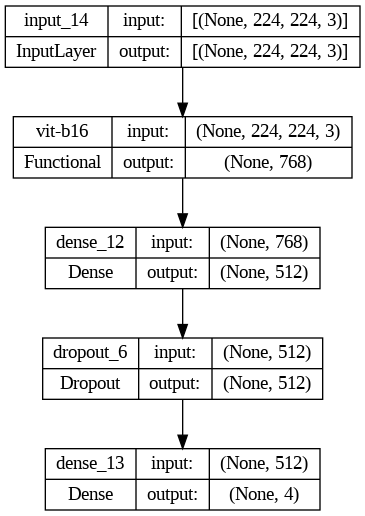
\includegraphics[width=0.45\textwidth]{vit/vit_architecture2.png}
  \caption{ViT Implemented Architecture}
  \label{fig:vit_implemented_architecture}
\end{figure}

Typically, the output layer of ViT uses a Multi-Layer Perceptron (MLP) layer as shown in Figure \ref{fig:vit_architecture}. However, since the dataset provided is very small and ViT models are generally used for very large datasets, a softmax activation function was used instead. The softmax function is advantageous in this context because it converts the output logits into probabilities that sum to one, which is particularly useful for multi-class classification problems. This provides a clear probabilistic interpretation of the model's predictions, making it easier to identify the most likely class for each input image. The final classification layer, therefore, utilizes a softmax activation function to provide the probabilities for each class, enhancing the model's ability to make accurate predictions on diverse MRI data.



The model training and optimization involved several critical steps. The model leverages a custom Adam optimizer with a learning rate of approximately 0.0001, based on its empirical effectiveness in similar tasks involving high-dimensional image data. This choice ensures stable and gradual adjustments to the weights. The categorical cross-entropy loss function was utilized to address the multi-class nature of the classification challenge, ensuring effective discrimination between different brain tumor types. 

To address class imbalance, a significant concern in medical datasets, the model training incorporated dynamically adjusted class weights. This strategy enhances the model's sensitivity to under-represented classes, thus improving its overall diagnostic accuracy. Training extended over 50 epochs with an early stopping mechanism that ceased training if there was no improvement in validation loss over 10 consecutive epochs. The optimal model was preserved and further assessed on a validation set, achieving a peak training accuracy of 0.9974 and a validation accuracy of 0.9111, with the lowest validation loss recorded at 0.33246.

The Vision Transformer (ViT) architecture, with its self-attention mechanisms, offers a robust and innovative approach for brain MRI classification. By leveraging the global context of images, the ViT model shows significant potential in enhancing the accuracy and reliability of medical image analysis, making it a valuable tool in the domain of medical diagnostics. The final model architecture consists of an input layer with dimensions 224x224x3, followed by the ViT-B16 functional layer, a dense layer with 512 neurons, a dropout layer, and a final dense layer with four neurons for classification. The total number of parameters in the model is 86,194,436, all of which are trainable.


\subsubsection{Fine-Tuning}


% TO MOD THIS %
% In the process of fine-tuning the model, the Optuna package was utilized to conduct a comparative analysis of different optimizers, namely RAdam, Adam, and SGD. This hyperparameter optimization process aimed to identify the most effective optimizer for the final model. After extensive experimentation, RAdam was selected due to its superior performance in achieving higher validation accuracy compared to the other optimizers. This choice aligns with the findings of Khaliki et al. \cite{khaliki_brain_2024}, which highlight the advantages of RAdam in stabilizing training and enhancing convergence rates.

% In addition to optimizer selection, the dropout rate was also a subject of optimization attempts using the Optuna package. Despite exploring various dropout rates, the optimal dropout rate was found to be 0.055, which provided a balance between mitigating overfitting and maintaining model performance. This specific dropout rate was thus adopted in the final model architecture.

% The overall approach demonstrates the rigorous method employed to fine-tune the model, ensuring optimal performance for brain tumor segmentation. By leveraging advanced optimization techniques and thoroughly validating the model, this work contributes to the development of more accurate and reliable medical imaging models.

\subsubsection{Results and Evaluation}


The confusion matrices in Figures \ref{fig:inceptionv3_cm1} and \ref{fig:inceptionv3_cm2}, provide a detailed view of the model's performance across the four brain tumor classes: meningioma, pituitary, glioma, and no tumor. The pituitary and no tumor classes exhibit slightly lower but still commendable true positive rates of 0.88, indicating strong performance across all categories. The classification report in Table \ref{tab:inceptionv3_classification_report} summarizes the precision, recall, and F1-score for each class. The model demonstrates high precision and recall across all classes, with a notable F1-score of 0.96 for the meningioma class. The overall micro, macro, and weighted averages for precision, recall, and F1-score all stand at 0.93, reflecting consistent and reliable performance.

The ROC curve in Figure \ref{fig:inceptionv3_roc} displays the true positive rate against the false positive rate for each class. The areas under the curve (AUC) for pituitary and no tumor classes are both perfect at 1.00, while meningioma and glioma classes show AUCs of 0.97 and 0.99, respectively, indicating excellent discriminative ability of the model.

The learning curve in Figure \ref{fig:inceptionv3_learning_curve} illustrates the model's accuracy and loss over 100 epochs. The convergence of training and validation accuracy, alongside the decreasing trend in loss values, indicates effective learning without significant overfitting.

Table \ref{tab:inceptionv3_additional_metrics} highlights the Dice Similarity Coefficient (DSC), sensitivity, specificity, and accuracy of the model. The DSC of 0.9272 indicates a high overlap between the predicted and actual tumor regions. Sensitivity and accuracy, both at 0.9271, demonstrate the model's ability to correctly identify true positives, while the specificity of 0.9757 shows its effectiveness in correctly identifying true negatives.

\subsubsection{K-Folds Cross-Validation}

K-Folds cross-validation was performed to evaluate the model's performance across different subsets of the dataset. The model achieved an average validation accuracy of 0.9711 and an average validation loss of 0.2188 across five folds. The model was trained for 90 epochs with a batch size of 10 for each fold. The results demonstrate the model's consistency and robustness in classifying brain tumor images.

Results from K-Folds cross-validation are summarized in Figure \ref{f:inceptionv3_kfolds}, illustrating the validation accuracy and loss for each fold. The consistent performance across all folds, with minimal variance in accuracy and loss values, further validates the model's reliability and effectiveness in brain tumor segmentation tasks.

% Validation Accuracy: 0.9711 ± 0.0218
% Validation Loss: 0.2188 ± 0.0586
% k = 5
% epochs = 90 
% batch_size = 10


\subsubsection{Conclusion}


